\documentclass[11pt, fleqn]{article}

\usepackage[usenames,dvipsnames,svgnames,table]{xcolor}
\usepackage{amsmath}
\usepackage{amsfonts}
\usepackage[margin=1in]{geometry} % To set the margin widths
\usepackage{graphicx}
\usepackage{listings}
\usepackage{multirow}
\usepackage{tabularx}
\usepackage{varioref}
\usepackage[noabbrev,capitalize]{cleveref}
\usepackage[group-separator={,}]{siunitx}
\usepackage{subcaption}
\usepackage{titlesec}
\usepackage{lscape}
\usepackage{bm}
\usepackage[titletoc,toc,title]{appendix}

\lstset{
  frame=single,
  basicstyle=\ttfamily,% print whole listing small
  language=R,
  aboveskip=3mm,
  belowskip=3mm,
  showstringspaces=false,
  columns=flexible,
  numbers=none,
  commentstyle=\color{ForestGreen},
  stringstyle=\color{Maroon},
  breaklines=true,
  breakatwhitespace=true,
  tabsize=2,
  literate={<-}{{$\gets$}}1 {~}{{$\sim$}}1
}

\sisetup{output-exponent-marker=\textsc{e}}

\setlength{\parskip}{12pt} % Sets a blank line in between paragraphs
\setlength\parindent{0pt} % Sets the indent for each paragraph to zero

\begin{document}

\title{Machine Learning (41204-01)\\HW \#6}
\author{Will Clark $\vert$ Matthew DeLio \\
\texttt{\{will.clark,mdelio\}@chicagobooth.edu} \\
University of Chicago Booth School of Business}
\date{\today}
\maketitle

\section{Data Summary}

The user that has rated the most video games is \texttt{U584295664}; he has rated 53 games. This user is an extreme outlier, as the median user rated only two games and only one other user rated more than 21 games. This behavior makes him approximately 22 standard deviations above the mean. We can see in \cref{fig:histo_users} just how extreme this outlier is (the maximum value is marked with a red line).

The game that has been rated most frequently is \texttt{I760611623}; it has been rated 200 times. This game is also an extreme outlier, as the median game has been rated three times and the next most-rated game was rated by only 102 users. The rating profile for this game puts it at approximately 15 standard deviations above the mean. We can see in \cref{fig:histo_games} how far from the center of the distribution this game is (the maximum value is again marked in red).

\begin{figure}
\centering
\begin{subfigure}[b]{0.49\textwidth}
\caption{by User}
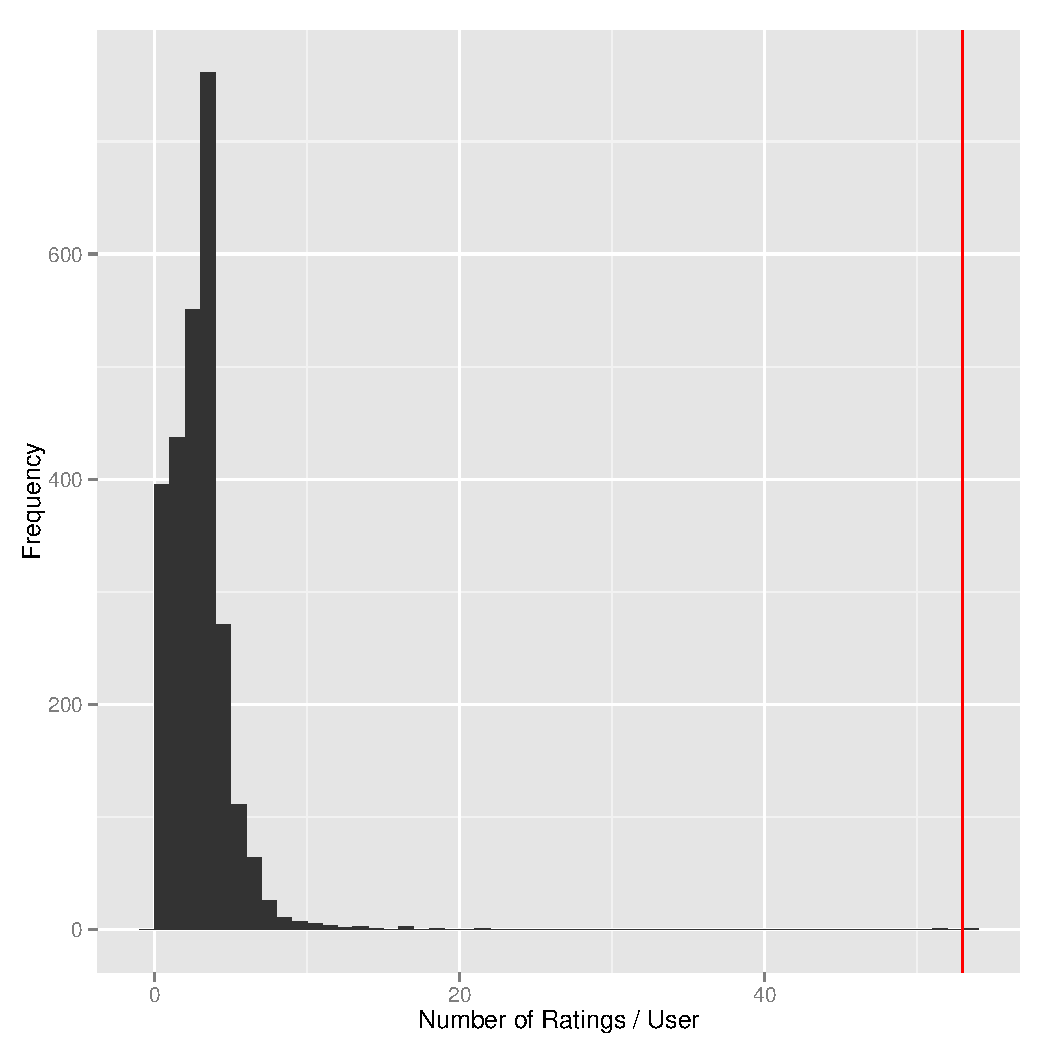
\includegraphics[width=\textwidth]{histo_users.pdf}
\label{fig:histo_users}
\end{subfigure}
\hfill
\begin{subfigure}[b]{0.49\textwidth}
\caption{by Game}
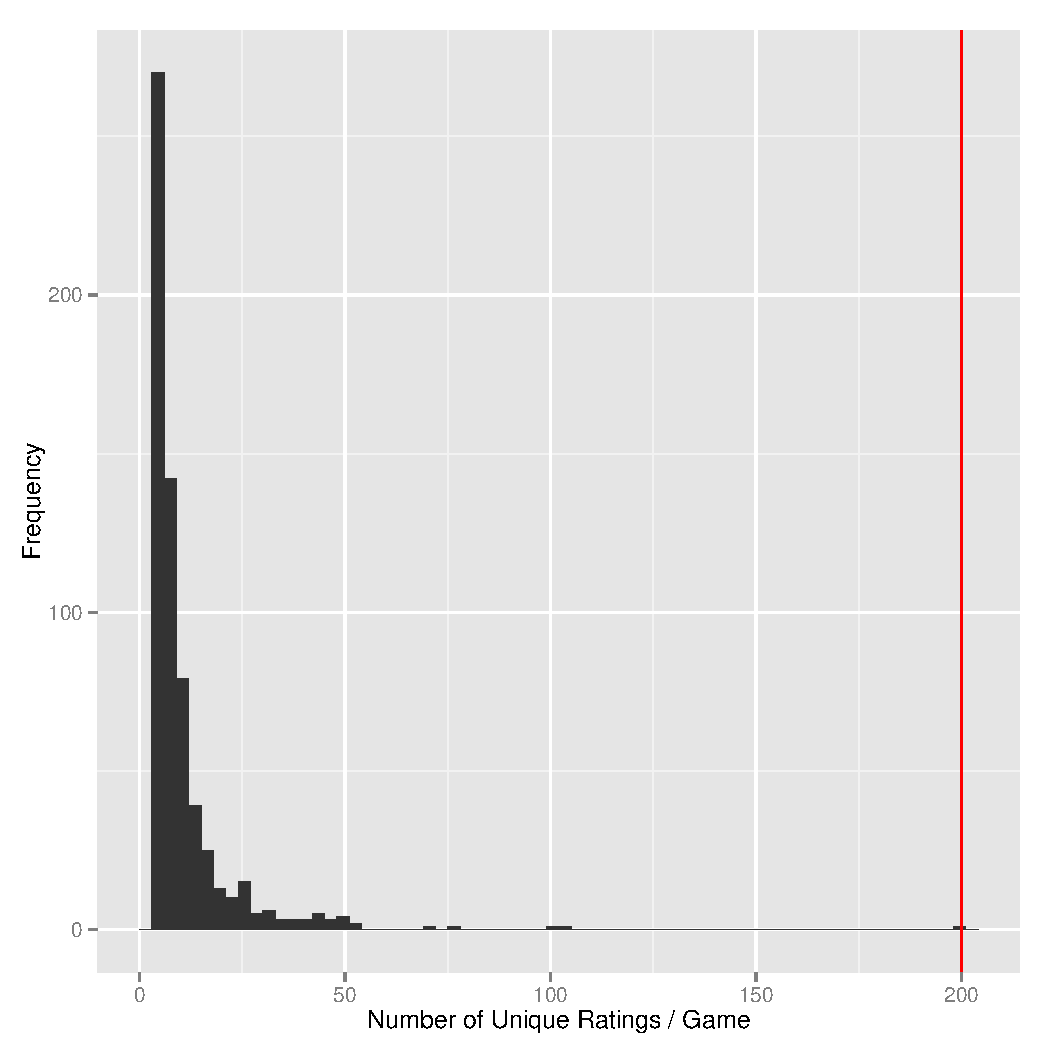
\includegraphics[width=\textwidth]{histo_games.pdf}
\label{fig:histo_games}
\end{subfigure}
\caption{Distribution of Rating Behavior}
\end{figure}

\section{User Similarity}
To find the user similarity


\section{Recommendations}



\begin{appendices}

\clearpage

%\section{Code Listings}
%\lstinputlisting[label=lst:code, caption=Code Snippet, language=R]{../hw5.R}

\end{appendices}

\end{document}

% \input{.tex}

% \begin{figure}
%   \centering
%   \begin{subfigure}[b]{0.49\textwidth}
%     \caption{}
%     \includegraphics[width=\textwidth]{.pdf}
%     \label{fig:}
%   \end{subfigure}
%   \hfill
%   \begin{subfigure}[b]{0.49\textwidth}
%     \caption{}
%     \includegraphics[width=\textwidth]{.pdf}
%     \label{fig:}
%   \end{subfigure}
%   \caption{}
% \end{figure}

% \begin{figure}[!htb]
%   \centering
%   \caption{}
%   \includegraphics[scale=.5]{.pdf}
%   \label{fig:}
% \end{figure}

